\subsection{嘉当子代数}

定义 1. 设 \(\mathfrak{g}\) 是一个李代数。\(\mathfrak{g}\) 的嘉当子代数是指 \(\mathfrak{g}\) 的一个等于其自身正规化子的幂零子代数。

后面我们将得到下列结果：

\begin{enumerate}
\def\labelenumi{\arabic{enumi})}
\item
  若 \(k\) 是无限的，则 \(\mathfrak{g}\) 有嘉当子代数（第 3 节，定理 1 的推论 1）；
\item
  若 \(k\) 的特征为零，则 \(\mathfrak{g}\) 的所有嘉当子代数都有相同的维数（§3，第 3 节，定理 2）；
\item
  若 \(k\) 是代数闭的且特征为 0，则 \(\mathfrak{g}\) 的所有嘉当子代数在 \(\mathfrak{g}\) 的初等自同构群下共轭（§3，第 2 节，定理 1）。
\end{enumerate}

例. 1) 若 \(\mathfrak{g}\) 幂零，则 \(\mathfrak{g}\) 的唯一嘉当子代数是 \(\mathfrak{g}\) 自身（第一章，§4，第 1 节，命题 3）。

\begin{enumerate}
\def\labelenumi{\arabic{enumi})}
\setcounter{enumi}{1}
\item
  设 \(\mathfrak{g} = \mathfrak{gl}(n,k)\) ，并设 \(\mathfrak{h}\) 是属于 \(\mathfrak{g}\) 的对角矩阵所成的集合。我们证明 \(\mathfrak{h}\) 是 \(\mathfrak{g}\) 的一个嘉当子代数。首先，\(\mathfrak{h}\) 是交换的，从而幂零。设 \((E_{ij})\) 是 \(\mathfrak{gl}(n,k)\) 的典则基，并设 \(x = \sum \mu_{ij}E_{ij}\) 是 \(\mathfrak{h}\) 在 \(\mathfrak{g}\) 中的正规化子的一个元素。若 \(i\neq j\) ，则第一章，§1，第 2 节的公式 (5) 表明 \(E_{ij}\) 在 \([E_{ii},x]\) 中的系数是 \(\mu_{ij}\) 。由于 \(E_{ii}\in \mathfrak{h}\) ，有 \([E_{ii},x]\in \mathfrak{h}\) ，故所述系数为零。于是 \(\mu_{ij} = 0\) 对 \(i\neq j\) 成立，从而 \(x\in \mathfrak{h}\) ，这表明 \(\mathfrak{h}\) 确是 \(\mathfrak{g}\) 的一个嘉当子代数。
\item
  设 \(\mathfrak{h}\) 是 \(\mathfrak{g}\) 的一个嘉当子代数，\(\mathfrak{g}_1\) 是 \(\mathfrak{g}\) 的一个包含 \(\mathfrak{h}\) 的子代数。那么 \(\mathfrak{h}\) 是 \(\mathfrak{g}_1\) 的一个嘉当子代数；这由定义 1 立即可得。
\end{enumerate}

命题 1. 设 \(\mathfrak{g}\) 是一个李代数，\(\mathfrak{h}\) 是 \(\mathfrak{g}\) 的一个嘉当子代数。那么 \(\mathfrak{h}\) 是 \(\mathfrak{g}\) 的一个极大幂零子代数。

设 \(\mathfrak{h}'\) 是 \(\mathfrak{g}\) 的一个包含 \(\mathfrak{h}\) 的幂零子代数。那么 \(\mathfrak{h}\) 是 \(\mathfrak{h}'\) 的一个嘉当子代数（例 3），故 \(\mathfrak{h} = \mathfrak{h}'\) （例 1）。

存在不是嘉当子代数的极大幂零子代数（习题 2）。

\pandocbounded{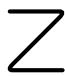
\includegraphics[keepaspectratio]{images/part001_35e3d035.jpg}}

命题 2. 设 \((\mathfrak{g}_i)_{i\in \mathrm{I}}\) 是李代数的一个有限族，且 \(\mathfrak{g} = \prod_{i\in \mathrm{I}}\mathfrak{g}_i\)

\(\mathfrak{g}\) 的嘉当子代数恰是形如 \(\prod_{i\in I}\mathfrak{h}_i\) 的子代数，其中 \(\mathfrak{h}_i\) 是 \(\mathfrak{g}_i\) 的嘉当子代数。

若 \(h_{i}\) 是 \(g_{i}\) 的一个以 \(n_{i}\) 为正规化子的子代数，则 \(\prod h_{i}\) 是 g 的一个以 \(\prod n_{i}\) 为正规化子的子代数；若诸 \(h_{i}\) 幂零，则 \(\prod h_{i}\) 幂零；于是，若对所有 i，\(h_{i}\) 都是 \(g_{i}\) 的嘉当子代数，则 \(\prod h_{i}\) 是 g 的嘉当子代数。反之，设 h 是 g 的一个嘉当子代数；投影 \(h_{i}\) （h 到 \(g_{i}\) 上的）是 \(g_{i}\) 的幂零子代数，且 \(\prod h_{i}\) 是 g 的包含 h 的幂零子代数；故 \(h = \prod h_{i}\) （命题 1）；于是对所有 i，\(h_{i}\) 是它在 \(g_{i}\) 中的自身的正规化子，从而是 \(g_{i}\) 的嘉当子代数。

例 4. 若 k 的特征为 0，则 \(\mathfrak{gl}(n,k)\) 是理想 \(\mathfrak{sl}(n,k)\) 与 k.1 的乘积。由例 2 与命题 2 可知，\(\mathfrak{sl}(n,k)\) 中迹为 0 的对角矩阵所成的集合是 \(\mathfrak{sl}(n,k)\) 的一个嘉当子代数。

命题 3. 设 g 是一个李代数，h 是 g 的一个子代数，\(k'\) 是 k 的一个扩张。那么 h 是 g 的嘉当子代数当且仅当 \(h \otimes_{k} k'\) 是 \(g \otimes_{k} k'\) 的嘉当子代数。

事实上，\(\mathfrak{h}\) 幂零当且仅当 \(\mathfrak{h} \otimes_k k'\) 幂零（第一章，§4，第 5 节）。另一方面，若 \(\mathfrak{n}\) 是 \(\mathfrak{h}\) 在 \(\mathfrak{g}\) 中的正规化子，则 \(\mathfrak{h} \otimes_k k'\) 在 \(\mathfrak{g} \otimes_k k'\) 中的正规化子是 \(\mathfrak{n} \otimes_k k'\) （第一章，§3，第 8 节）。

命题 4. 设 \(\mathfrak{g}\) 是一个李代数，\(\mathfrak{h}\) 是 \(\mathfrak{g}\) 的一个幂零子代数。那么 \(\mathfrak{h}\) 是 \(\mathfrak{g}\) 的嘉当子代数当且仅当 \(\mathfrak{g}^0 (\mathfrak{h}) = \mathfrak{h}\) 。

若 \(\mathfrak{g}^0 (\mathfrak{h}) = \mathfrak{h}\) ，则 \(\mathfrak{h}\) 是它自身的正规化子（§1，命题 10 (i)），故 \(\mathfrak{h}\) 是 \(\mathfrak{g}\) 的嘉当子代数。假定 \(\mathfrak{g}^0 (\mathfrak{h})\neq \mathfrak{h}\) 。考虑由伴随表示转到商而得到的 \(\mathfrak{h}\) 在 \(\mathfrak{g}^0 (\mathfrak{h}) / \mathfrak{h}\) 上的表示。应用 Engel 定理（第一章，§4，第 2 节，定理 1），可见存在 \(x\in \mathfrak{g}^0 (\mathfrak{h})\) 使得 \(x\notin \mathfrak{h}\) 且 \([\mathfrak{h},x]\subset \mathfrak{h}\) ；于是 \(x\) 属于 \(\mathfrak{h}\) 在 \(\mathfrak{g}\) 中的正规化子，故 \(\mathfrak{h}\) 不是 \(\mathfrak{g}\) 的嘉当子代数。

推论 1. 设 \(\mathfrak{g}\) 是一个李代数，\(\mathfrak{h}\) 是 \(\mathfrak{g}\) 的一个嘉当子代数。若 \(k\) 是无限的，则存在 \(x \in \mathfrak{h}\) 使 \(\mathfrak{h} = \mathfrak{g}^0(x)\) 。

事实上，\(\mathfrak{h} = \mathfrak{g}^0 (\mathfrak{h})\) ，故可应用 §1 的命题 9 (ii)。

推论 2. 设 \(f: \mathfrak{g} \to \mathfrak{g}'\) 是李代数的满射同态。若 \(\mathfrak{h}\) 是 \(\mathfrak{g}\) 的嘉当子代数，则 \(f(\mathfrak{h})\) 是 \(\mathfrak{g}'\) 的嘉当子代数。

事实上，\(f(\mathfrak{h})\) 是 \(\mathfrak{g}'\) 的幂零子代数。另一方面，考虑表示 \(x \mapsto \operatorname{ad} f(x)\) ，即 \(\mathfrak{h}\) 在 \(\mathfrak{g}'\) 上的表示。由 §1 第 3 节的命题 9 (iv)，\(f(\mathfrak{g}^0(\mathfrak{h})) = \mathfrak{g}'^0(\mathfrak{h})\) 。而 \(\mathfrak{g}^0(\mathfrak{h}) = \mathfrak{h}\) ，另一方面显然有 \(\mathfrak{g}'^0(\mathfrak{h}) = \mathfrak{g}'^0(f(\mathfrak{h}))\) 。于是 \(f(\mathfrak{h}) = \mathfrak{g}'^0(f(\mathfrak{h}))\) ，只需应用命题 4。

推论 3. 设 \(\mathfrak{h}\) 是李代数 \(\mathfrak{g}\) 的一个嘉当子代数，并设 \(\mathcal{C}^n\mathfrak{g}\) （ \(n \geq 1\) ）是 \(\mathfrak{g}\) 的下降中心列的一项（第一章，§1，第 5 节）。那么 \(\mathfrak{g} = \mathfrak{h} + \mathcal{C}^n\mathfrak{g}\) 。

事实上，推论 2 表明 \(\mathfrak{h}\) 在 \(\mathfrak{g} / \mathcal{C}^n\mathfrak{g}\) 中的像是 \(\mathfrak{g} / \mathcal{C}^n\mathfrak{g}\) 的嘉当子代数，由于 \(\mathfrak{g} / \mathcal{C}^n\mathfrak{g}\) 幂零（例 1），故它等于 \(\mathfrak{g} / \mathcal{C}^n\mathfrak{g}\) 。

推论 4. 设 \(\mathfrak{g}\) 是一个李代数，\(\mathfrak{h}\) 是 \(\mathfrak{g}\) 的一个嘉当子代数，\(\mathfrak{a}\) 是 \(\mathfrak{g}\) 的一个包含 \(\mathfrak{h}\) 的子代数。

\begin{enumerate}
\def\labelenumi{(\roman{enumi})}
\item
  \(\mathfrak{a}\) 等于它在 \(\mathfrak{g}\) 中的自身的正规化子。
\item
  假定 \(k = \mathbf{R}\) 或 \(\mathbf{C}\) ；设 \(G\) 是以 \(\mathfrak{g}\) 为李代数的一个李群，A 是 \(G\) 的以 \(\mathfrak{a}\) 为李代数的积分子群。那么 \(A\) 是 \(G\) 的一个李子群，且它是 \(A\) 在 \(G\) 中的正规化子的单位元连通分支。
\end{enumerate}

设 n 是 a 在 g 中的正规化子。由于 h 是 n 的嘉当子代数（例 3），\(\{0\}\) 是 n/a 的嘉当子代数（推论 2），故等于它在 n/a 中的正规化子；换言之，n = a。断言 (ii) 由 (i) 及第三章，§9，第 4 节，命题 11 的推论得出。

推论 5. 设 g 是一个李代数，E 是 g 的一个子集。让 E 通过伴随表示作用在 g 上。那么 E 是 g 的嘉当子代数当且仅当 \(E = \mathfrak{g}^{0}(E)\) 。

该条件是必要的（命题 4）。现在假定 \(\mathrm{E} = \mathfrak{g}^0 (\mathrm{E})\) 。由 §1 第 1 节的命题 2 (ii)，E 这时是 \(\mathfrak{g}\) 的一个子代数。若 \(x\in \mathrm{E}\) ，则 \(\mathrm{ad}_{\mathrm{E}}x\) 幂零，由于 \(\mathrm{E}\subset \mathfrak{g}^0 (\mathrm{E})\) ；故代数 E 幂零。于是由命题 4，E 是嘉当子代数。

推论 6. 设 g 是一个李代数，\(k_{0}\) 是 k 的一个使 \([k:k_{0}]<+\infty\) 的子域，\(g_{0}\) 是由 g 把纯量域限制到 \(k_{0}\) 而得到的李代数。设 h 是 g 的一个子集。那么 h 是 g 的嘉当子代数当且仅当 h 是 \(g_{0}\) 的嘉当子代数。

这由推论 5 得出，因为条件 \(\mathfrak{h} = \mathfrak{g}^0 (\mathfrak{h})\) 与基域无关。

命题 5. 设 g 是一个李代数，c 是它的中心，h 是 g 的一个向量子空间。那么 h 是 g 的嘉当子代数当且仅当 h 包含 c 且 h/c 是 g/c 的嘉当子代数。

假定 \(\mathfrak{h}\) 是 \(\mathfrak{g}\) 的嘉当子代数。由于 \([\mathfrak{c},\mathfrak{g}]\subset \mathfrak{h}\) ，有 \(\mathfrak{c}\subset \mathfrak{h}\) 。另一方面，由命题 4 的推论 2，\(\mathfrak{h} / \mathfrak{c}\) 是 \(\mathfrak{g} / \mathfrak{c}\) 的嘉当子代数。

假定 \(\mathfrak{h} \supset \mathfrak{c}\) 且 \(\mathfrak{h} / \mathfrak{c}\) 是 \(\mathfrak{g} / \mathfrak{c}\) 的嘉当子代数。设 \(f\) 是从 \(\mathfrak{g}\) 到 \(\mathfrak{g} / \mathfrak{c}\) 的典则态射。代数 \(\mathfrak{h}\) 是 \(\mathfrak{h} / \mathfrak{c}\) 的一个中心扩张，故幂零。设 \(\mathfrak{n}\) 是 \(\mathfrak{h}\) 在 \(\mathfrak{g}\) 中的正规化子。若 \(x \in \mathfrak{n}\) ，则 \([f(x), \mathfrak{h} / \mathfrak{c}] \subset \mathfrak{h} / \mathfrak{c}\) ，故 \(f(x) \in \mathfrak{h} / \mathfrak{c}\) ，从而 \(x \in \mathfrak{h}\) 。这证明 \(\mathfrak{h}\) 是 \(\mathfrak{g}\) 的嘉当子代数。

推论. 设 \(\mathcal{C}_{\infty}\mathfrak{g}\) 是李代数 \(\mathfrak{g}\) 的上升中心列的并（第一章，§1，第 6 节）。\(\mathfrak{g}\) 的嘉当子代数恰是 \(\mathfrak{g}/\mathcal{C}_{\infty}\mathfrak{g}\) 的嘉当子代数的逆像。

事实上，\(\mathfrak{g} / \mathcal{C}_i\mathfrak{g}\) 的中心是 \(\mathcal{C}_{i + 1}\mathfrak{g} / \mathcal{C}_i\mathfrak{g}\) ，用归纳法由命题 5 立即得出该推论。

注. \(C_{\infty}g\) 是使 g/n 的中心为零的最小理想 n；它是 g 的一个特征幂零理想。

